\subsection{Model-complexity and model-selection}


In this section we try to compare the performances of the Perceptron, we implemened during the first assignment against the SVM from this one.
Since the Perceptron can only handle linearly separable data, we will use a SVM with hard margin and linear Kernel for this comparison.
\\
\\
To select a proper test set we selected $M = 150$ training sets $\tau _{k},k \in \{1,\ldots,M\}$ form the MNIST training set with no more than $N = 70$ images each.
For $k \in \{1,\ldots,M\}$ we trained both SVM and Perceptron using $\tau_k$ and calculated the test error rate $R_k = \sum_{i=1}^{n}( (t_{i}^{\ast} - \hat{t_{i}} )^2 * \frac{1}{4n} ) $ on the {MNIST} test set - again for both SVM and Perceptron.
\\
\\
The average error $R_{avg} = \frac{1}{M}\sum_{k=1}^M R_k$ of SVM and Perceptron can be seen in the table below (Table \ref{tab:avg_error}).
Figure \ref{fig:error_SVM_perc} shows $\tau_k$ with the error rate for $\tau_k$.\\

As we can see performs the SVM already better than the Perceptrom, which still has to be verified.
%Against our expectations SVM does not perform as well as suspected, which could be due to the use of the linear Kernel and $C=\infty$ (no slack variables).
%Otherwise we would have suspeceted the SVM would have found a decision boundary similar or better than Perceptron.

\begin{table}[!h]
 \begin{center}
\begin{tabular}{|c|c|}
 \hline
 \textbf{$R_{avg}$ SVM} & \textbf{ $R_{avg}$ Perceptron} \\
 \hline
 0.01441156462585034       &     0.027952380952380954      \\
 \hline
\end{tabular}
\caption{\label{tab:avg_error} $R_{avg}$ for both algorithms }
\end{center}
\end{table}

\begin{figure}[!h]
\begin{center}
\centering
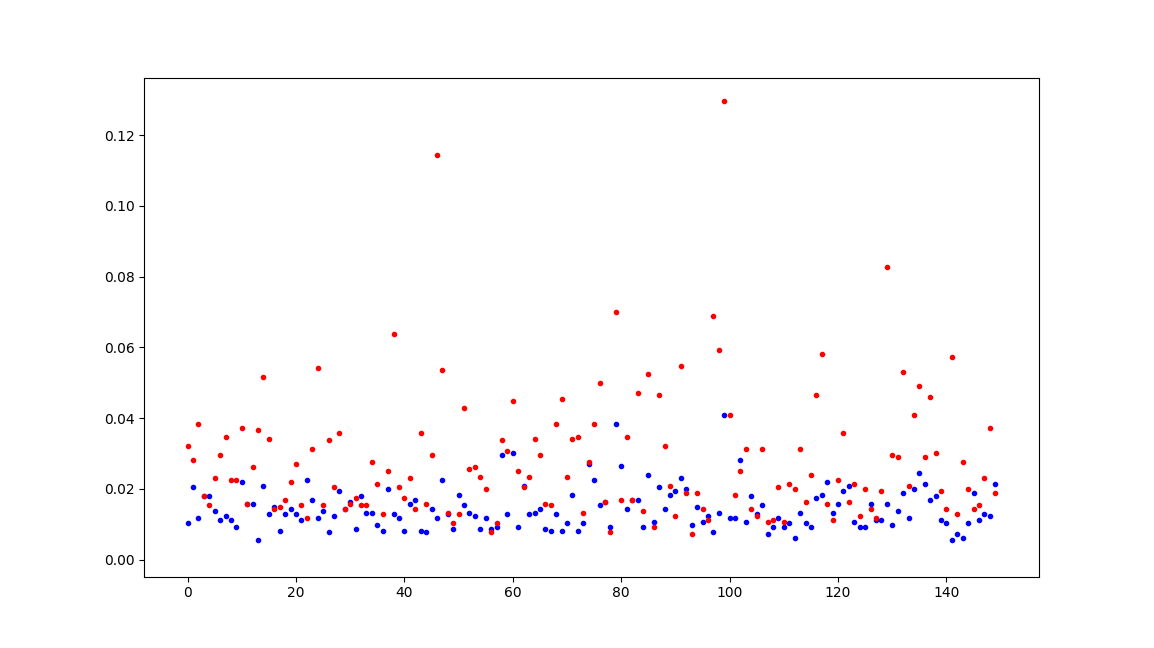
\includegraphics[width=1\textwidth]{figures/perc_svn_comparison.png}
\end{center}
\caption{\label{fig:error_SVM_perc} Comparing the error rates of $\tau_k$ from SVM (blue) against Perceptron(red) }
\end{figure}



\subsection{Tuning meta-parameters $C$ and $\sigma$}

This last section describes the effects of changing $C$ and $\sigma$ when using a RBF-kernel. In general $C$, a slack varibale, allows to not meet the margin requirement at a cost proportional to a value, which still allows us to minimize the error, but relaxes the stiffnes of linear separability.


\begin{figure}[!h]
\begin{center}
\centering
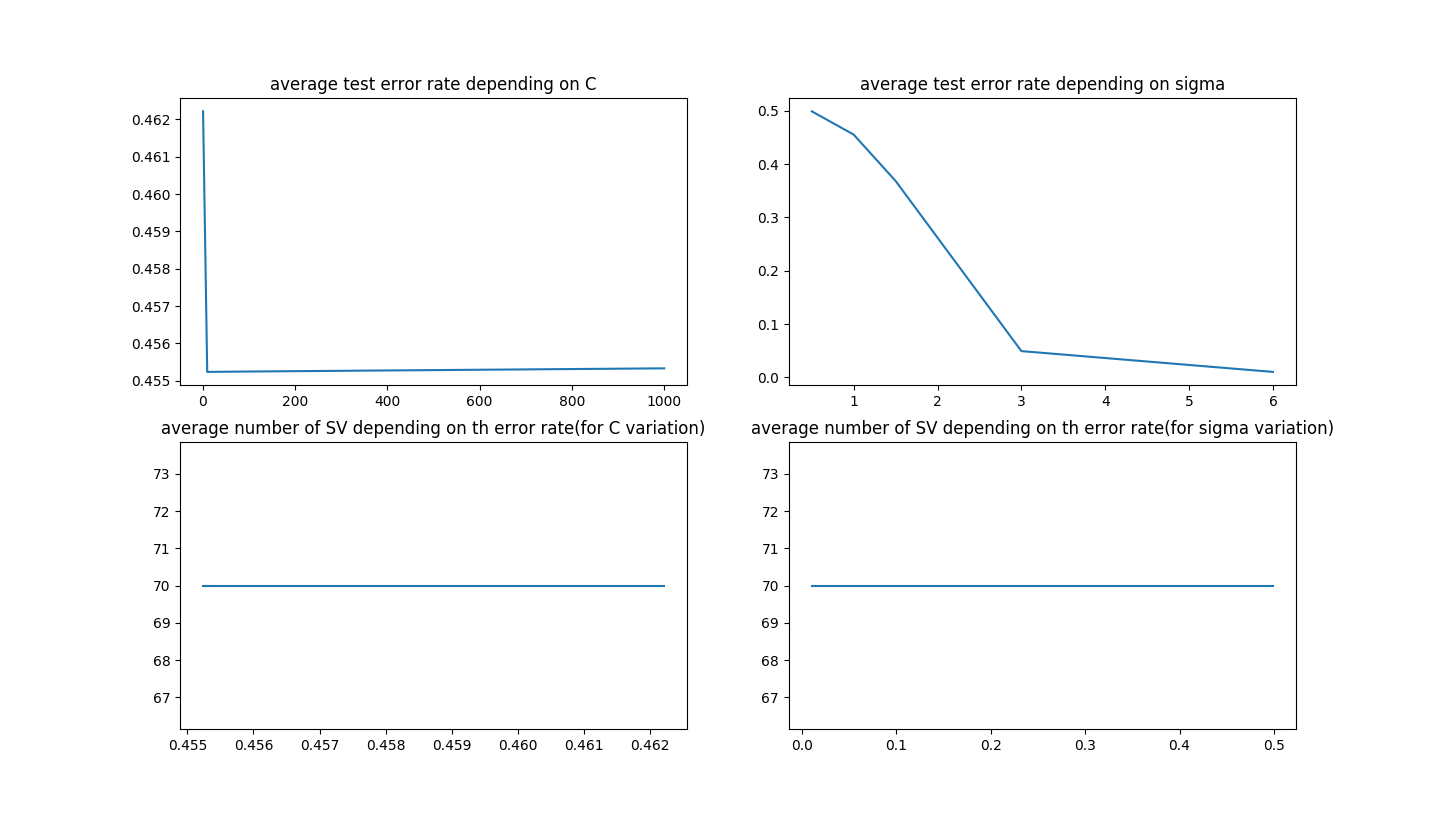
\includegraphics[width=1\textwidth]{figures/avg_test_error.png}
\end{center}
\caption{\label{fig:error_avg_erros} }
\end{figure}





